\documentclass[12pt]{article}

\usepackage{xltxtra}
\usepackage{graphicx}
\usepackage{setspace}
\usepackage{minted}
\usepackage{hyperref}
\usepackage[magyar]{babel}

\hypersetup{
  bookmarks=true,
  unicode=true,
  pdftitle={Node.js backend multiplayer játékhoz},
  pdfauthor={Dányi Bence},
  pdfcreator={Dányi Bence},
  pdfproducer={XeLaTeX},
  pdfkeywords={node.js, websocket, redux, canvas, flowtype, babel},
  pdfnewwindow=true,
  colorlinks=true,
  linkcolor=black,
  citecolor=black,
  filecolor=black,
  urlcolor=black
}

\newminted[js]{javascript}{fontsize=\footnotesize}

\setlength{\parindent}{0pt}
\setlength{\parskip}{8pt plus 3pt minus 3pt}
\onehalfspacing

\begin{document}
\begin{titlepage}
  \begin{center}
    
\includegraphics[width=0.5\textwidth]{figures/logo}~\\[1cm]
    \textsc{Budapesti Műszaki és Gazdaságtudományi Egyetem}
    \\[1.5cm]
    \textsc{\Large Önálló Laboratórium 2.}
    \\[1cm]
    { \huge \bfseries Node.js backend multiplayer játékhoz }
    \\[2cm]

    \noindent
    \begin{minipage}[t]{0.4\textwidth}
      \begin{flushleft}
        \large
        \emph{Készítette:}\\
        \textsc{Dányi} Bence
    \end{flushleft}
    \end{minipage}%
    \begin{minipage}[t]{0.4\textwidth}
      \begin{flushright}
        \large
        \emph{Konzulens:} \\
        \textsc{Imre} Gábor
      \end{flushright}
    \end{minipage}

    \vfill

    {\large \today}
  \end{center}
\end{titlepage}
\section{A feladat}

A félév során elvégzendő feladat egy több szereplős játék elkészítése volt,
mely során az én feladatom a játék logikájának megtervezése és implementálása,
valamint a kliens és a szerver közötti kommunikáció megvalósítása volt.

A játékban a játékosok egy űrhajót irányítanak a billentyűzet segítségével,
amivel az űrhajó hajtóműveit tudják ki és bekapcsolni.
A játék célja a többi játékos kiiktatása, ezt az űrhajóra szerelt fegyverekkel
lehet megtenni.

\section{Felhasznált techonlógiák}

Az elkészült alkalmazás ES2015 \cite{es2015} nyelven készült el, ez a JavaScript 2015 nyarán
szabványosított változata. A szerver NodeJS \cite{node} környezetben fut, így a kliens és
a szerver nagy arányban használja ugyanazt a kódot.

A kliens-szerver kommunikáció Websocket \cite{websocket} technológián alapul.
Számos absztrakció létezik a kommunikáció részleteinek elfedésére (EngineIO, Primus),
én azonban az overhead elkerülése végett ezeket nem használtam, pusztán
a natív Websocket API-ra.

A szerver oldali kiszolgálást a \texttt{koa}\cite{koa} webszerver végzi, ami a népszerű \texttt{express}\cite{express}
szerver következő generációs verziója. A modul API-ja könnyen olvasható,
a kiszolgálásért ún. middleware-ek felelősek. Ezek aszinkron módon működnek,
amit a koa egy generátor alapú megoldással tesz kényelmessé.
Hagyományosan a nyelvben az aszinkron műveletek eredménye (vagy sikertelensége)
egy ún. callback függvényben kezelhető le (hasonlóan a Java/C\#-ban ismert eseménykezelőkhöz),
ezt egyszerűsíti le a generátor alapú szintaxis, ami a C\#-ban meglévő \texttt{async/await}\cite{csasync}
konstrukciónak felel meg. Jó hír, hogy a nyelv következő változata (ES2016) már
tartalmazni fog egy hasonló konstrukciót\cite{jsasync}.
Mivel az alkalmazás kódját a Babel transpiler fordítja le futtatható JavaScript
kódra, így ez a kényelmes konstrukció már elérhető volt számomra is.

\subsection{Babel}

A Babel\cite{babel} (korábban 6to5\cite{6to5}) egy ún. transpiler, azaz olyan compiler, amiben a forrás
és a célnyelv ugyanaz. A feladata a böngészők (illetve a NodeJS futtatókörnyezet)
által még nem futtatható JavaScript kód (ES2015) transzformálása egy korábbi,
általánosan elérhető dialektusra (ES5).

Mivel az alkalmazás moduláris felépítésű, így szükség van az elkészült állományok
összecsomagolására, ez a böngésző számára a hatékonyabb betöltés miatt szükséges.
Ezt könnyíti meg a \texttt{browserify}\cite{browserify} csomag, ami a forrásfájlokból egyetlen, a kliens
által futtatható \emph{bundle}-t csinál.
Fejlesztés közben a teljes fordítás sajnos nagyon lassú (ahogy minden más nyelvben),
így a folyamat felgyorsítására a \texttt{watchify}\cite{watchify} csomagot használtam, ami \emph{inkrementális}
fordítást biztosít, illetve folyamatosan figyeli a forrásfájlokat,
így a fordítás automatikus.

\subsection{Flowtype}

A JavaScript nyelv egyik nagy hátrányának a statikus típusosság hiányát tartják.
Erre nyújt megoldás a Facebook techonlógiája, a Flowtype\cite{flowtype}, mely a nyelvet
új nyelvi elemekkel (\emph{típusannotációkkal}) egészíti ki, és lehetőséget ad a program
típushelyességének bizonyítására, mindezt a fordítási folyamat részeként.

A típusellenőrzés opcionális, a \texttt{@flow} direktívával engedélyezhető, így alkalmas
fokozatos bevezetésre már meglévő projectekben is.
A fordító fejlett (a \emph{Hindley-Milner}\cite{hindley-milner} típusrendszert használja), képes az egyes típusok kikövetkeztetésére, így elegendő
a függvény szignatúráját (valójában elég csak a modulból kiexportált függvények
szignatúráját) annotálni, a többi típus kikövetkeztethető (típus inferencia).

\subsection{redux}

A \texttt{redux}\cite{redux} egy állapot-konténer melynek segítségével a fejlesztő egyszerűen képes
az alkalmazás állapotát (\texttt{store}) egy egységes \emph{API}-n keresztül módosítani.
A felhasználó akciókat süt el, melynek hatására a felület frissül.
Az akciók egyszerű Javascript objektumok, egy kötelező \texttt{type} tulajdonsággal,
egy opcionális \texttt{payload} és egy szintén opcionális \texttt{meta} propertyvel ellátva.

A type az akció típusát tartalmazza, erre azért van szükség, hogy a sorosítás
során (amire a Websocket kapcsolat miatt van szükség) ne vesszen el
típusinformáció.
A \texttt{payload} az akcióhoz kapcsolódó adatokat (paramétereket) tartalmazza,
ha van ilyen, akkor az tipikusan egy hagyományos JavaScript objektum (de
természetesen tetszőleges egyéb primitív típus is lehet).
A \texttt{meta} az akcióhoz szorosan nem kapcsolódó információkat tartalmazza, tipikusan
szintén egy JavaScript objektum.
Az alkalmazásban a szerverre felküldendő akciók \texttt{pending: true} propertyvel
váltódnak ki, így azok nem közvetlenül a kliensen hajtódnak végre, hanem
Websocket kapcsolaton keresztül a szerveren futnak le (ami tipukusan visszaküldi az
akciót már a pending property nélkül).

A kiváltott akciót a \texttt{store} \texttt{dispatch} metódusával tudjuk aktiválni,
amit a központ alkalmazáslogika egy \texttt{(state, action) => state} típusú
függvénnyel kezel le. A \texttt{redux} ezt a logikai elemet \emph{reduce}-nek hívja,
a JavaScriptből ismert \texttt{reduce} függvényhez hasonló működése miatt (más funkcionális nyelvekben
ez a \texttt{fold} függvénynek felel meg).

Mielőtt az egyek akciók eljutának a központi alkalmazáslogikáig, lehetőség van
azokat \emph{elkapni}, azokat módosítani, tetszőleges műveletet végezni rajtuk ún. \emph{middleware}-ekkel.
Az játákban a szerveren végrehajtandó akciókat is egy ilyen middleware kapja el,
amiket aztán továbbít a WebSocket kapcsolatok keresztül.

\section{Az elkészült alkalmazás}

A játéknak az elosztott adatbázisok tipikus problémáját kell megoldania:
megfelelő reszponzivitást nyújtani a konzisztencia megtartása mellett.
Mivel mind a szerver, mind a kliens JavaScript-ben van írva, így a játéklogika
mind a szerveren, mind a kliensen egyszerre (párhuzamosan) fut,
köztük a megfelelő szinkronizációt kellett csak megoldani.
Ez az üzenetek mennyiségét tekintve egy nagyon hatákony megoldás, hiszen amíg
felhasználói interakció nem történik a játékban, addig mind a szerver, mind a
kliens azonos állapotot lát (hiszen a szimuláció teljesen determinisztikus).

A játék állapotát akciók kiváltásával lehet megváltoztatni, ezek az akciók
mindig a felhasználótól erednek, így akciókat csak a kliensek tudnak kiváltani.
Jelenleg a támogatott akciók a hajók vezérlésével kapcsolatosak (hajtóművek ki
és bekapcsolása, fegyverek elsütése, játékhoz csatlakozás, játék elhagyása).

A kliens által kiváltott akciók nem megbízhatóak, mivel a kód a kliens kontrollja alatt áll:
adott esetben illegális műveleteket hajthatna végre (más játékos avatarjának irányítása, stb.).
Ennek megelőzésére a szerver a kiváltott akciókon validálást végez (azaz vizsgálja,
hogy az akció a játék szabályainak megfelel-e).
Ha az akció végrehajtható, a szerver minden csatlakozott játékosnak elküldi
a végrehajtott akciót, akik a saját lokális játék-példányukat annak megfelelően módosítják.
Ezt a működést mutatja be \aref{fig:ws-arch}. ábra.

\begin{figure}[h!]
  \centering
  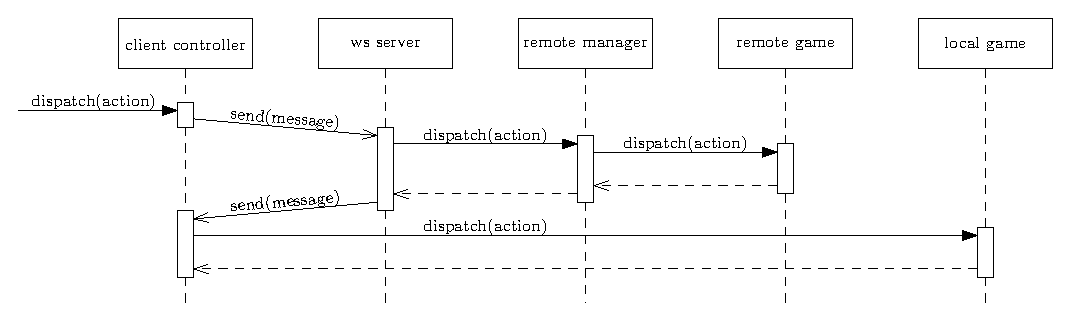
\includegraphics[width=\textwidth]{figures/ws}
  \caption{A Websocket alapú kommunikáció architektúrája}
  \label{fig:ws-arch}
\end{figure}

A játéklogika alapvetően két részből áll: első lépésben az objetktumokat a fizika
törvényeinek megfelelően mozgatni és forgatni kell, majd az akciót ténylegesen végrehajtani.
Az objektumok mozgásának szimulációja a diszkrét szimulációs módszeren alapszik,
az egyes entitások minden egyes időszeletben (az időszelet hossza konfigurálható,
a gyakorlatban a $20ms$ elegendően részletesnek bizonyult) egyenletesen gyorsuló
mozgást végez:

\[
  F_e = \sum_{i=0}^nF_i
\]

\begin{js}
  const netForce = object.forces.reduce(
    (force, f) => add(force, f),
    { x: 0, y: 0 }
  );
\end{js}

\[
  M_e = \sum_{i=0}^n(r_i - R) \times F_i
\]

\begin{js}
  const netTorqe = object.forces.reduce(
    (torqe, f) => torqe + cross(f.position, unit(f.orientation)) * f.strength,
    0
  );
\end{js}

Minden hajóra $F_e$ eredő erő hat, illetve $M_e$ forgatónyomaték hat az $R$ pontban
(ahol $r_i$ az $i$-edik hajtómű helyzete, $F_i$ az álatala kifejtett erő, $R$ pedig a hajó aktuális pozíciója).
Az erők alapján a szimuláció Euler integrálással történik, ami a ténylegeses lejátszódó
folyamatnak csak egy durva közelítése, azonban a gyakorlatban elegendően pontosnak bizonyult.
A szimuláció pszeudokódja ezek alapján a következő:

\begin{js}
  const comp = (f, g) => ((s, a) => g(f(s, a), a));
  const reduce = comp(
    (state, action) => {
      while (state.time < action.time) {
        state = evolve(state, dt);
      }
      return state;
    },

    (state, action) => {
      return handleUserInput(state, action);
    }
  );
\end{js}

A \texttt{comp} függvény a függvénykompozícióhoz hasonló működést implementál,
feladata a két szimulációs lépés összekapcsolása. Az első lépés felelős azért,
hogy a virtuális világ szinkronban legyen a kiválasztott akcióval, amit a második
lépésben alkalmaz az aktuális állapotra.

Az így létrejött \texttt{reduce} függvény egy determinisztikus függvény,
ami a komplett játéklogikát magában foglalja.

A megoldás előnye, hogy \emph{pure function}, azaz nem módosítja a bemeneti
változókat, a visszatérési értéke pedig csak a bemeneti változóktól függ,
így nagyon jól tesztelhető: gyors, mivel nem végez költséges IO műveleteket,
nem igényel bonyolult \emph{setup} és \emph{teardown} folyamatokat, egyszerűen
a kimenet vizsgálatával eldönthető a működés helyessége.

\subsection{Perzisztens adatstruktúrák}

Az alkalmazás kliens oldali részének állapotát egy egyszerű objektum-gráf
reprezentálja, a kiváltott akciók ezt az állapotot befolyásolják.
Azoban az állapot közvetlenül nem módosítható, minden akció egy teljesen
új állapotot eredményez. Ez nem jelenti azt, hogy minden egyes akció lekezelésekor
le kellene másolni a meglévő állapot, annak pusztán a megváltozott részét szükséges
legyártani, a többi részét a gráfnak hivatkozni lehet (hiszen az nem változhat meg később sem).

Ez azt eredményezi, hogy az alkalmazás állapota könnyen elmenthető és visszaállítható
tetszőleges pontra. Mivel a gráf minden eleme egy egyszerű JavaScript objektum,
így az állapot sorosítható is (akár localStorage-ba is, így bezárás után is képes megtartani az állapotát).

\section{Továbbfejlesztési lehetőségek}

A játék grafikája jelenleg nagyon sematikus, ezen rengeteg dolog javítható,
egy érdekes feladat lenne valamilyen WebGL-es megoldással 3 dimenziós grafikát
adni hozzá.

A játék irányítása sajnos nem túl intuitív, a hajtóművek szabályozása nagyon
nehéz. Ez egy teljesen szándékos döntés, a későbbiekben szeretnék implementálni
egy scriptelési réteget a vezérlés fölé, azaz a játékosok az űrhajó API-ját
felhasználva egy teljesen testreszabható szabályozási rendszert építhet fölé
(akár intuitívabb vezérlést, de akár egy komplett mesterséges intelligenciát).
Később a játékosok akár meg is tudnák ezeket a vezérlőket osztani egymással.

\begin{thebibliography}{9}
  \bibitem{es2015}
  Ecma International, \emph{ECMAScript® 2015 Language Specification},
  \url{http://www.ecma-international.org/ecma-262/6.0/ECMA-262.pdf}

  \bibitem{node}
  \emph{NodeJS}, \url{https://nodejs.org}

  \bibitem{websocket}
  I. Fette, A. Melnikov,
  \emph{The WebSocket Protocol}
  \url{https://tools.ietf.org/rfc/rfc6455.txt}

  \bibitem{koa}
  \emph{Koa - next generation web framework for node.js}
  \url{http://koajs.com/}

  \bibitem{express}
  \emph{Fast, unopinionated, minimalist web framework for Node.js}
  \url{http://expressjs.com/}

  \bibitem{csasync}
  \emph{Asynchronous Programming with Async and Await}
  \url{https://msdn.microsoft.com/en-us/library/hh191443.aspx}

  \bibitem{jsasync}
  \emph{Async Functions}
  \url{http://tc39.github.io/ecmascript-asyncawait/}

  \bibitem{babel}
  Babel
  \url{http://babeljs.io}

  \bibitem{6to5}
  James Kyle, \emph{Not Born to Die}
  \url{http://babeljs.io/blog/2015/02/15/not-born-to-die/}

  \bibitem{browserify}
  James Halliday, \emph{Browserify} \url{http://browserify.org/}

  \bibitem{watchify}
  James Halliday, \emph{watchify} \url{http://npmjs.com/watchify}

  \bibitem{flowtype}
  Facebook, \emph{Flowtype} \url{http://flowtype.org}

  \bibitem{hindley-milner}
  Hindley, J. Roger \emph{The Principal Type-Scheme of an Object in Combinatory Logic}, 1969

  \bibitem{redux}
  Dan Abramov, \emph{redux} \url{http://rackt.org/redux/}

\end{thebibliography}

A hivatkozott internetes források, ha az másként nincs jelölve, elérhetőek voltak ekkor: \today

\end{document}
